\documentclass[a4paper]{article}

%% Language and font encodings
\usepackage[english]{babel}
\usepackage[utf8x]{inputenc}
\usepackage[T1]{fontenc}

%% Sets page size and margins
\usepackage[a4paper,top=3cm,bottom=2cm,left=3cm,right=3cm,marginparwidth=1.75cm]{geometry}

%% Useful packages
\usepackage{listings}
\usepackage{algorithm}
\usepackage[noend]{algpseudocode}
\usepackage{float}
\usepackage{amsmath,bm,mathrsfs}
\usepackage{amsthm,amssymb}
\usepackage{graphicx}
%\usepackage[draft]{graphicx}
\usepackage[colorinlistoftodos]{todonotes}
\usepackage[colorlinks=true, allcolors=blue]{hyperref}

%% Operators
\newcommand{\R}{\mathcal{R}}
\newcommand{\RR}{\mathbb{R}}
\newcommand{\N}{\mathbb{N}}
\newcommand{\G}{\mathcal{G}}
\newcommand{\V}{\mathcal{V}}
\newcommand{\E}{\mathcal{E}}
\newcommand{\La}{\mathcal{L}}
\newcommand{\UR}{U_{\mathcal{R}}}
\newcommand{\vv}{\mathit{v}}
\renewcommand{\l}{\ell}

\theoremstyle{definition}
\newtheorem*{definition}{Definition}
\newtheorem*{thm}{Theorem}

\title{Notes}

\begin{document}
\maketitle

\newpage


\section{Things to fix:}
\begin{enumerate}
\item (fixed) Undefined function 'findpeaks' for input
arguments of type 'double'.

Error in mcsfb\_design\_filter\_bank\_no\_fourier
(line 31)
    [~, idx] = findpeaks(inverted); 
    
\item (fixed) Warning: Matrix is close to singular or badly scaled (Reconstruction using eigenvalue and eigenvectors)


\item filter design function - does not perform well

\end{enumerate}

\section{Notations}
Consider a weighted, undirected graph $\G = \{ \V, \E, W\}$, where $\V$ is the set of $N$ vertices, $\E$ is the set of edges and $W$ is the associated weighted adjacency matrix. Let $D$ be the diagonal matrix of vertex degrees. Denote $\La$ as the graph Laplacian, where $\La = D-W$. Since $\La$ is real, symmetric and semi-definite, we can diagonalize it as $\La =U\Lambda U^*$, where $\Lambda$ is the diagonal matrix of its real eigenvalues $\lambda_0, \lambda_1,\cdots, \lambda_{N-1}$ and the columns $u_0, u_1 \cdots u_{N-1}$ of $U$ are corresponding orthonormal eigenvectors of $\La$. We use $\UR$ to denote the submatrix formed by taking the columns of $U$ associated with the Laplacian eigenvalues indexed by $\mathcal{R} \subseteq \{0,1,\cdots,N-1\}$. And we use $U_{\mathcal{S},\mathcal{R}}$ to denote the submatrix formed by taking the rows of $U_{\mathcal{R}}$ associated with the vertices indexed by the set $\mathcal{S} \subseteq \{1,2,\cdots, N\}$. For $i \in \{1,\cdots,n\}$, $\bm{\delta_i} \in \RR^n$ denotes the $i$th column of the identity matrix $I \in \RR^{n\times n}.$
We consider graph signals $f \in \RR^N$ residing on a graph $\G$. A signal $f \in \RR^n$ defined on the nodes of the graph $\G$ is $\R$-concentrated if $f \in \text{span}(U_{\R})$. The graph Fourier transform of a signal is $\hat{f} = U*f$ and $\hat{g}(\La) f = U\hat{g}(\Lambda)U*f$ filters a graph signal by $\hat{g}(\cdot)$. Signal $r\in \RR^N$ is a random vector such that each entry is randomly draw from a standard gaussian distribution.

\medskip

\section{Definitions}
%\begin{definition}
%A signal $\bm{x} \in \RR^n$ defined on the nodes of the graph $\G$ is $k$-bandlimited with $k \in \N^+$ if $\bm{x} \in \text{span}(U_{\R})$ and $|\R| = k$.
%\end{definition}

\begin{definition}
A signal $\bm{f} \in \RR^n$ defined on the nodes of the graph $\G$ is $\R$-concentrated if $\bm{f} \in \text{span}(U_{\R})$.
\end{definition}

\begin{definition}
Let $\bm{p} \in \RR^{n}$ represent a sampling distribution on $\{1,2,\cdots n\}$. The graph weighted coherence of order $|\R| $ for the pair $(\G, \bm{p})$ is
$$ \vv^k_{\bm{p}} = \underset{1\leq i\leq n}{\text{ max }} \{\bm{p_i}^{-1/2} ||U_{\R}^T \bm{\delta_i} ||_2\}$$

\end{definition}

\section{Theorems}
\begin{thm}[Orthogonality Proof]

Let $\{\R_1, \R_2, \cdots, \R_M\}$ be $M$ partitions of the graph Laplacian eigenvalue indices $\{0, 1, \cdots,  N \}$ and $\{g_1, g_2, \cdots, g_M \}$ be filters defined on each of the $M$ bands. Then, the subspace spanned by $g_i(\La)$ is orthogonal to the subspace spanned by $g_j(\La)$ for $i \neq j$

\end{thm}

\begin{proof}


Notice that the $(i,j)$ entry of matrix $g(\La)$ can be represented as 

$$g(\La) (i,j) = [Ug(\Lambda)U^T] (i,j) = \sum_{k = 1}^{N} g(\lambda_k) U_k(i) U_k(j)$$

Now consider two filters $g_1$ and $g_2$. To show that two subspaces spanned are orthogonal, we show that the dot product of any two vectors is 0.
\begin{align*}
g_1(\La)(,k) \cdot g_2(\La)(,l)&=\ \  \sum_{j = 1}^{N} [\sum_{k = 1}^{N} g_1(\lambda_k) U_k(i) U_k(j) )( \sum_{l = 1}^{N} g_2(\lambda_l) U_l(i) U_l(j)) ] \\
& = \sum_{k = 1}^{N} \sum_{l = 1}^{N} g_1(\lambda_k) g_2(\lambda_l)  U_k(i) U_l(i) ( \sum_{j = 1}^{N}  U_k(j)  U_l(j))  \\
& = \sum_{k = 1}^{N} g_1(\lambda_k) g_2(\lambda_k)  U_k(i) U_k(i) ( \sum_{j = 1}^{N}  U_k(j)  U_k(j)) 
\end{align*}

Notice that $g_1(\lambda_k) g_2(\lambda_k)$ is always equal to $0$, since $g_1$ and $g_2$ are defined on disjoint sets of Laplacian eigenvalues.   

\end{proof}



%\begin{proof}

%$$g_1(\La) = Ug_1(\Lambda)U^T$$

%$$g_2(\La) = Ug_2(\Lambda)U^T$$

%Notice that $g_1(\lambda_k) g_2(\lambda_k)$ is always equal to $0$, since $g_1$ and $g_2$ are defined on disjoint sets of Laplacian eigenvalues.  
%\end{proof}
%\end{comment}


\newpage

\section{Abstract}
     We investigate an $M$-channel critically sampled filter bank for graph signals where each of the $M$ filters is supported on a different subband of the graph Laplacian spectrum. For analysis, on each subband, the graph signal is filtered using efficient polynomial approximation methods and then downsampled on a corresponding set of vertices chosen via non-uniform random sampling. We use an efficient decoder derived from the non-uniform sampling distribution to reconstruct the filtered signals on each band from their samples. We leverage an approximation of the spectral density function of the graph Laplacian to both approximate the number of eigenvalues in each band and design the filter bank to be more amenable to polynomial approximation, in order to reduce the resulting reconstruction error. We empirically explore the joint vertex-frequency localization of the dictionary atoms, the sparsity of the analysis coefficients, and the ability of the proposed transform to compress piecewise-smooth graph signals. 



\section{Filter Bank Design}

In order to circumvent expensive full eigendecompositions used to design ideal filter banks, we adopt the tight warped filter bank design discussed in \cite{shuman2013spectrum} to build a scalable filter bank of $M$ graph spectral filters. The tight warped filter bank design can be adapted to the width of the spectrum using only an estimate of the maximum eigenvalue and the filters can then be applied using the polynomial approximation methods discussed in \cite{hammond2011wavelets, shuman_DCOSS_2011}.

In this section, we construct the approximated filter bank of $M$ filters, where each filter is stored as the coefficients of Chebyshev or Jackson-Chebyshev polynomial approximations. In order to minimize the error caused by approximated filtering, we try to set the band ends between the spectral gaps. There are four steps toward building a filter bank, which are detailed below.

\subsection{Approximate Spectral Density Function}

Various methods have been proposed by past literature to approximate the distributions of eigenvalues. \cite{hammond2011wavelets,shuman_DCOSS_2011} uses the diagonal decomposition of shfited spectrum to count the number of eigenvalues in the shifted band. {\color{red}TODO: add more sources}

In our implementation,  we use the trace approximation method developed in \cite{approximating spectral densities of large matrices}. Given a filter $\hat{g}(\cdot)$, we notice that $\hat{g}(\La)$ is a diagonal matrix, where $\hat{g}(\La)_{i,i} = 1$ if the $i$th eigenvalues is covered by the filter and $\hat{g}(\La)_{i,i} = 0$ otherwise. By computing the trace of $\hat{g}(\La)$, which is the sum of the diagonal, we can obtain the number of eigenvalues in the band specified by $\hat{g}(\cdot)$. This method is of $\Theta(N)$ time complexity.
In practice, the trace can be approximated using the following fact:
\begin{align*}
tr(\hat{g}(\La)) &= E[r^T\hat{g}(\La)r] \\
&\propto \frac{1}{I}\sum_{i =1}^{I} (r^{i})^T\hat{g}(\La)r^{i}\\
\end{align*}


\subsection{Approximate Filtering}

When selecting the band ends for each of the $M$ ideal filters, we consider two factors: spectrum-adaptation and band spacing method. In our implementation, the filter bank can be either spectrum-adapted or not, and it can be either evenly spaced or logarithmic spaced. With the approximated CDF and PDF of Laplacian eigenvalues, we can set band ends according to these two parameters. All four possibilities are illustrated in the figure below:

\begin{figure}[h]
\centering
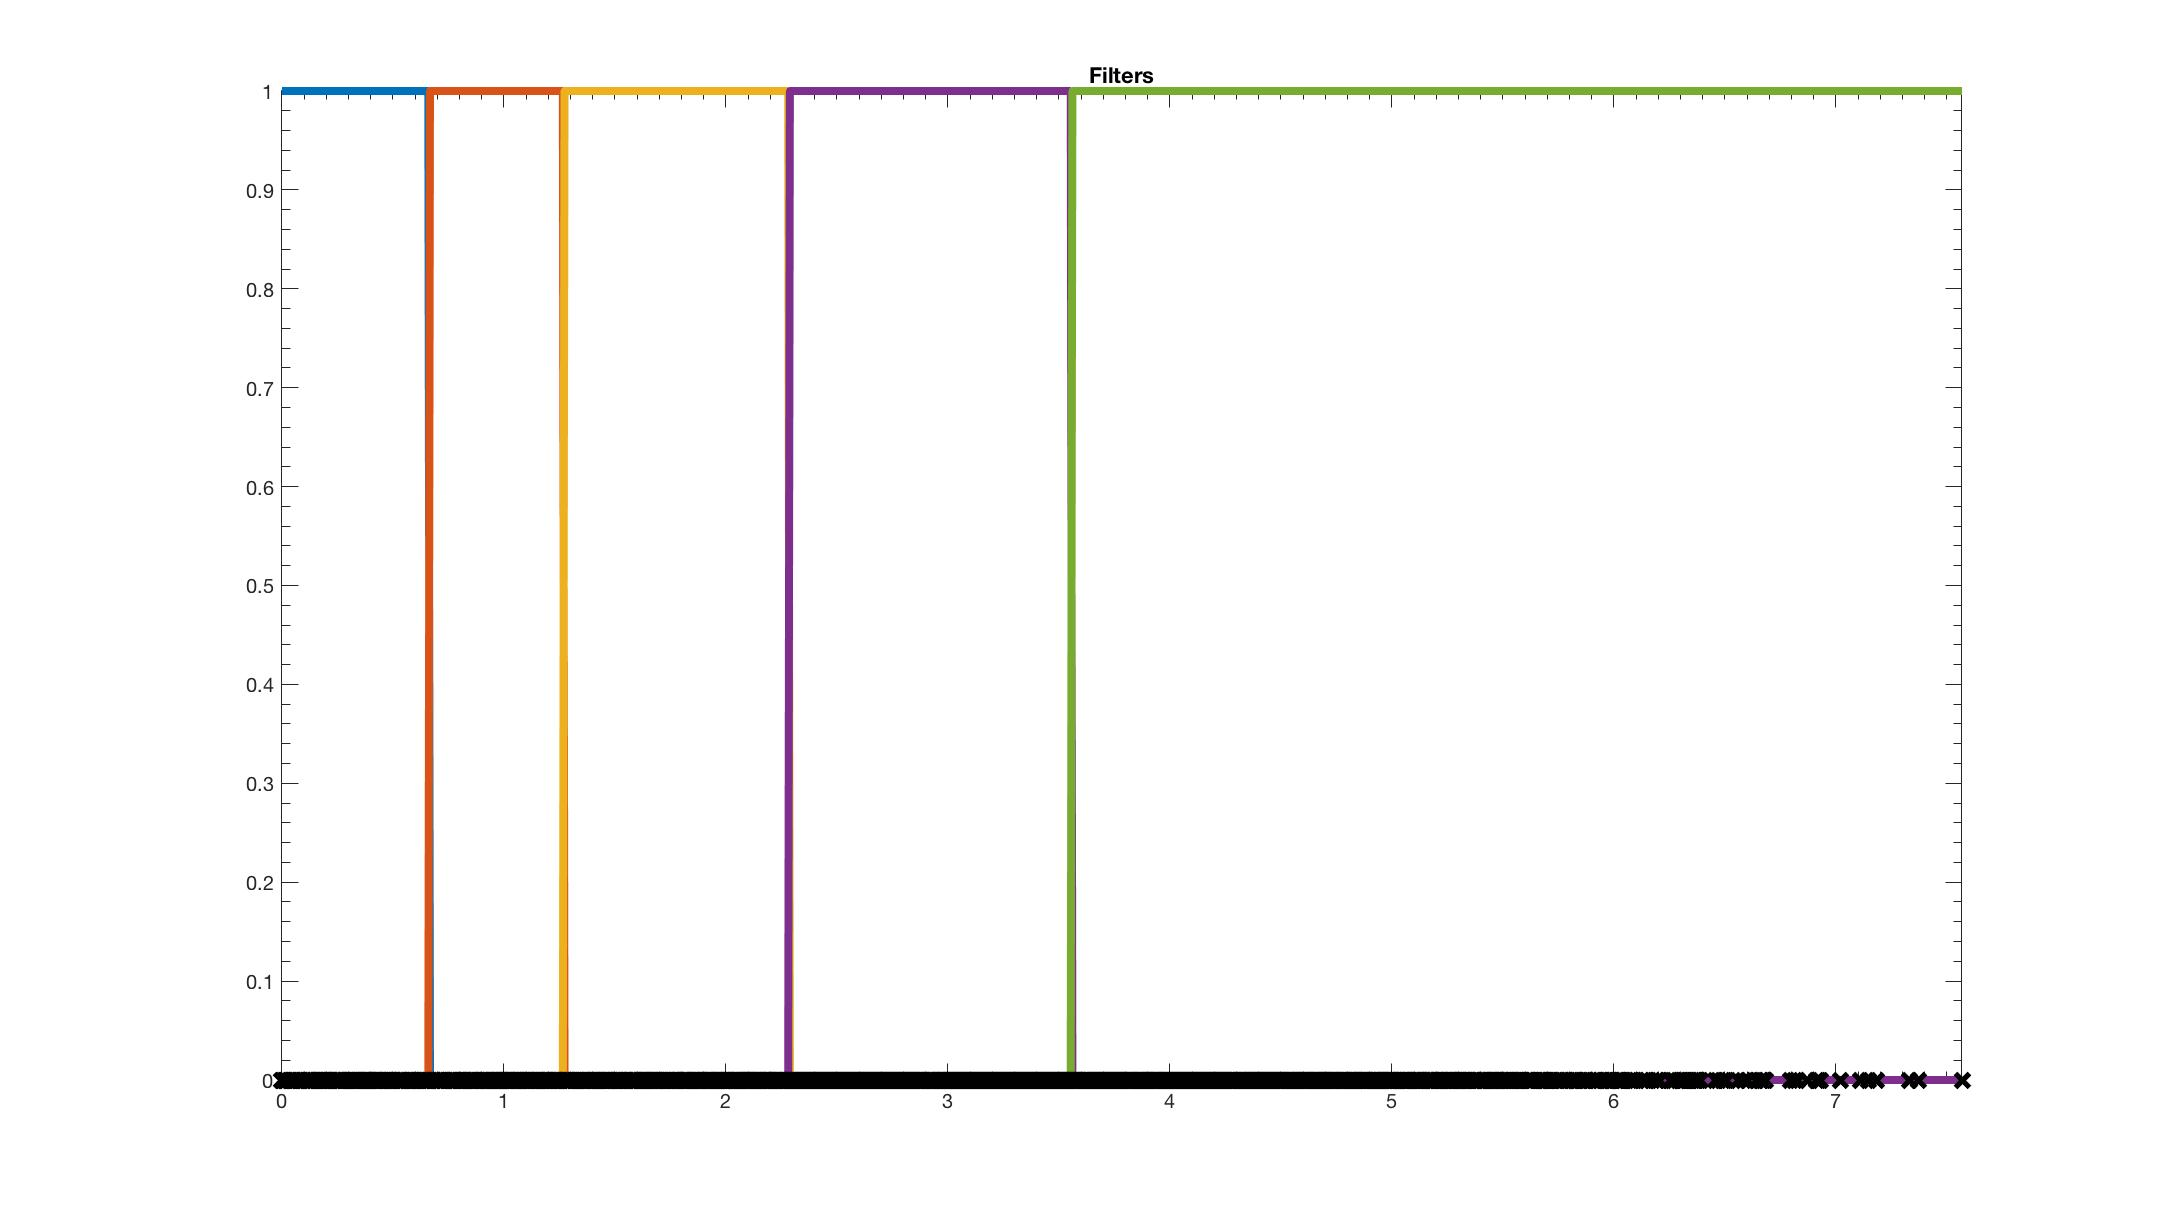
\includegraphics[width = 5cm]{filter_bank_1}
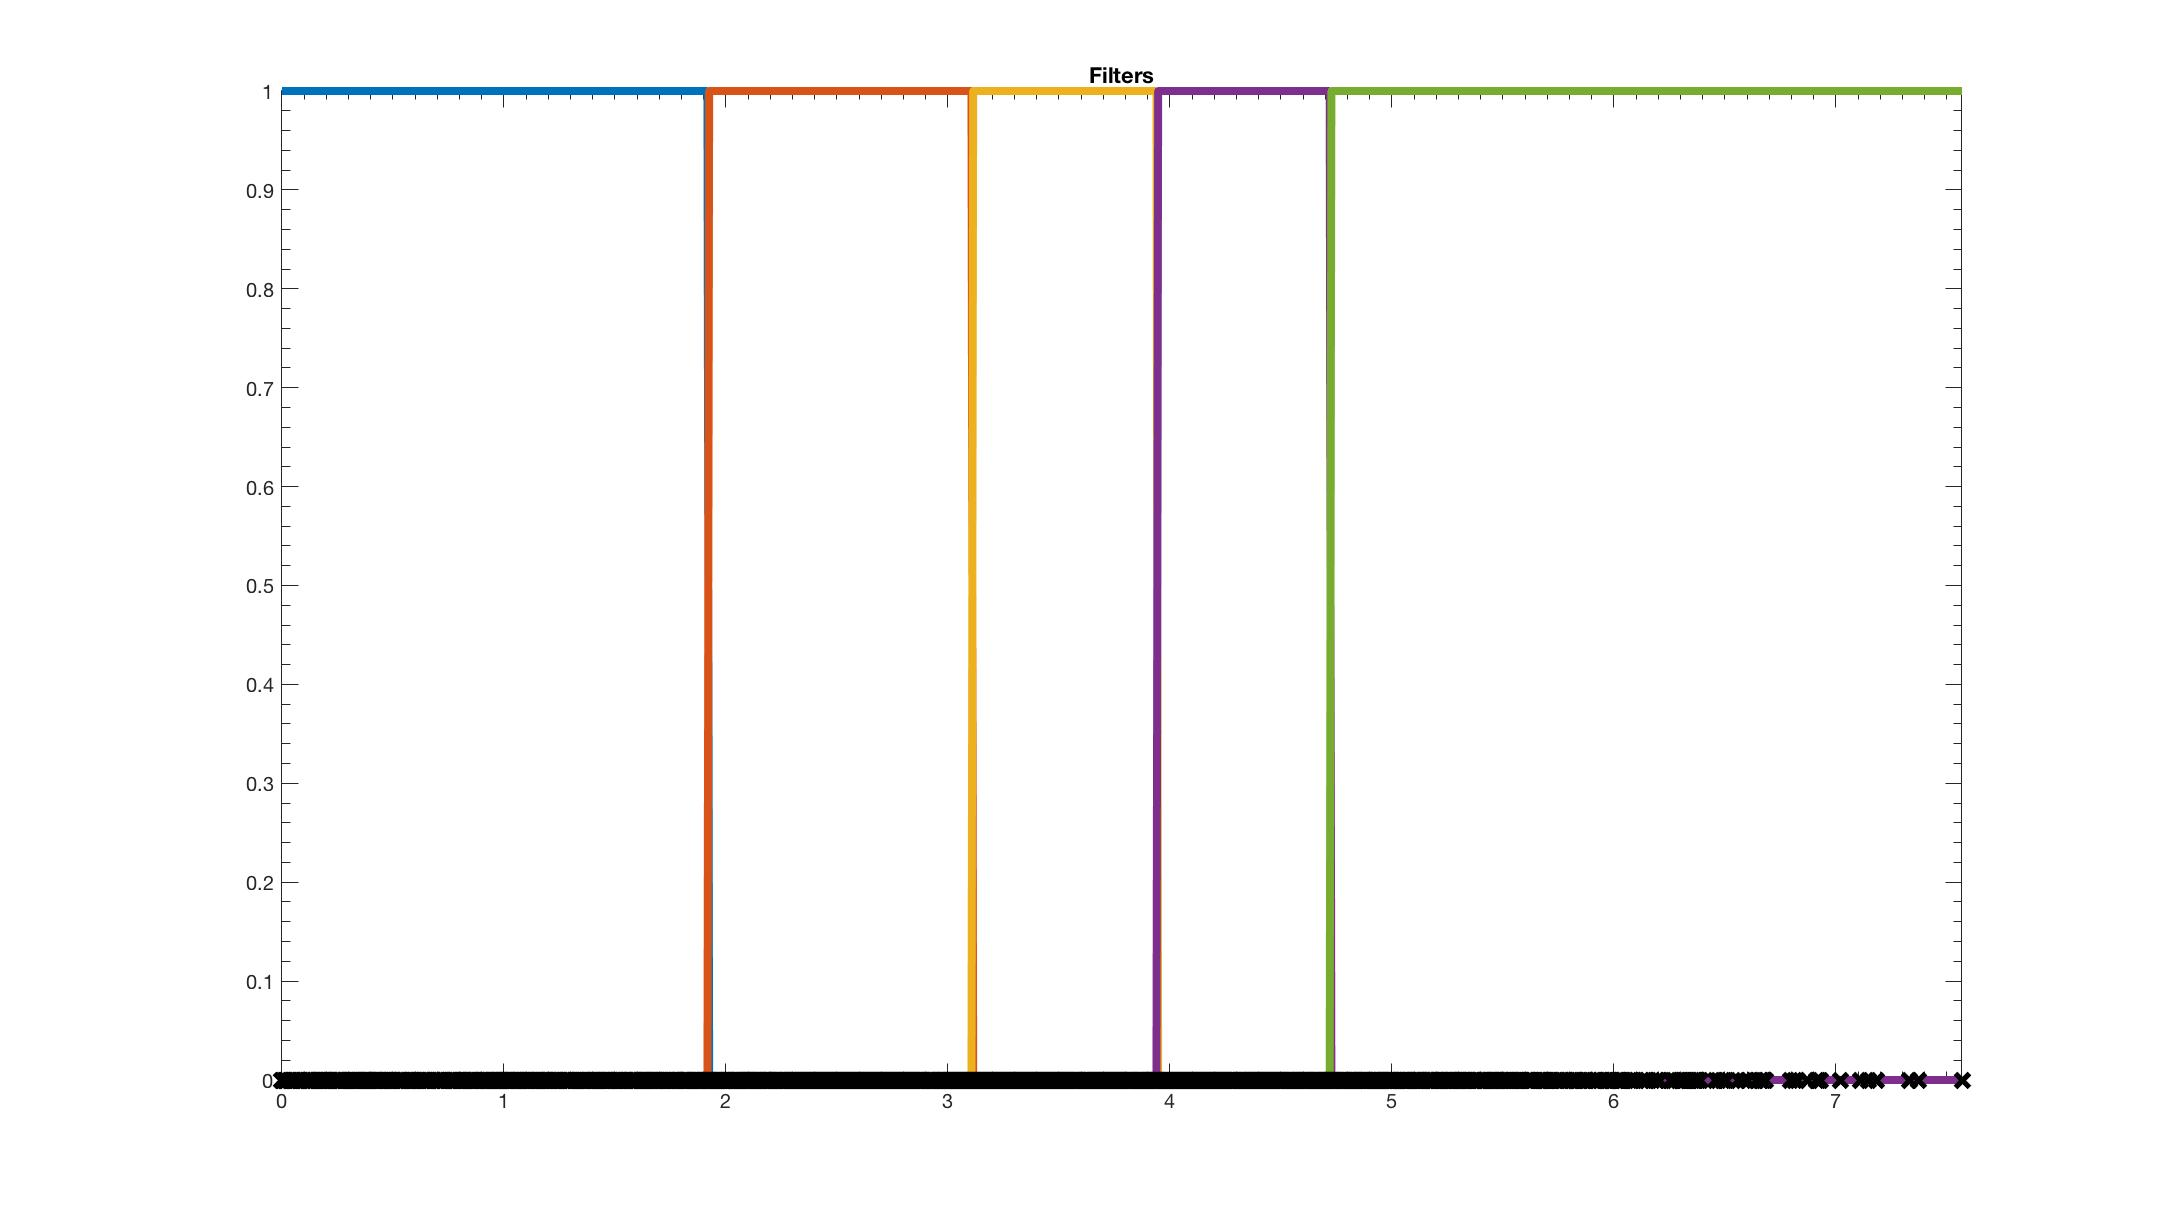
\includegraphics[width = 5cm]{filter_bank_2}

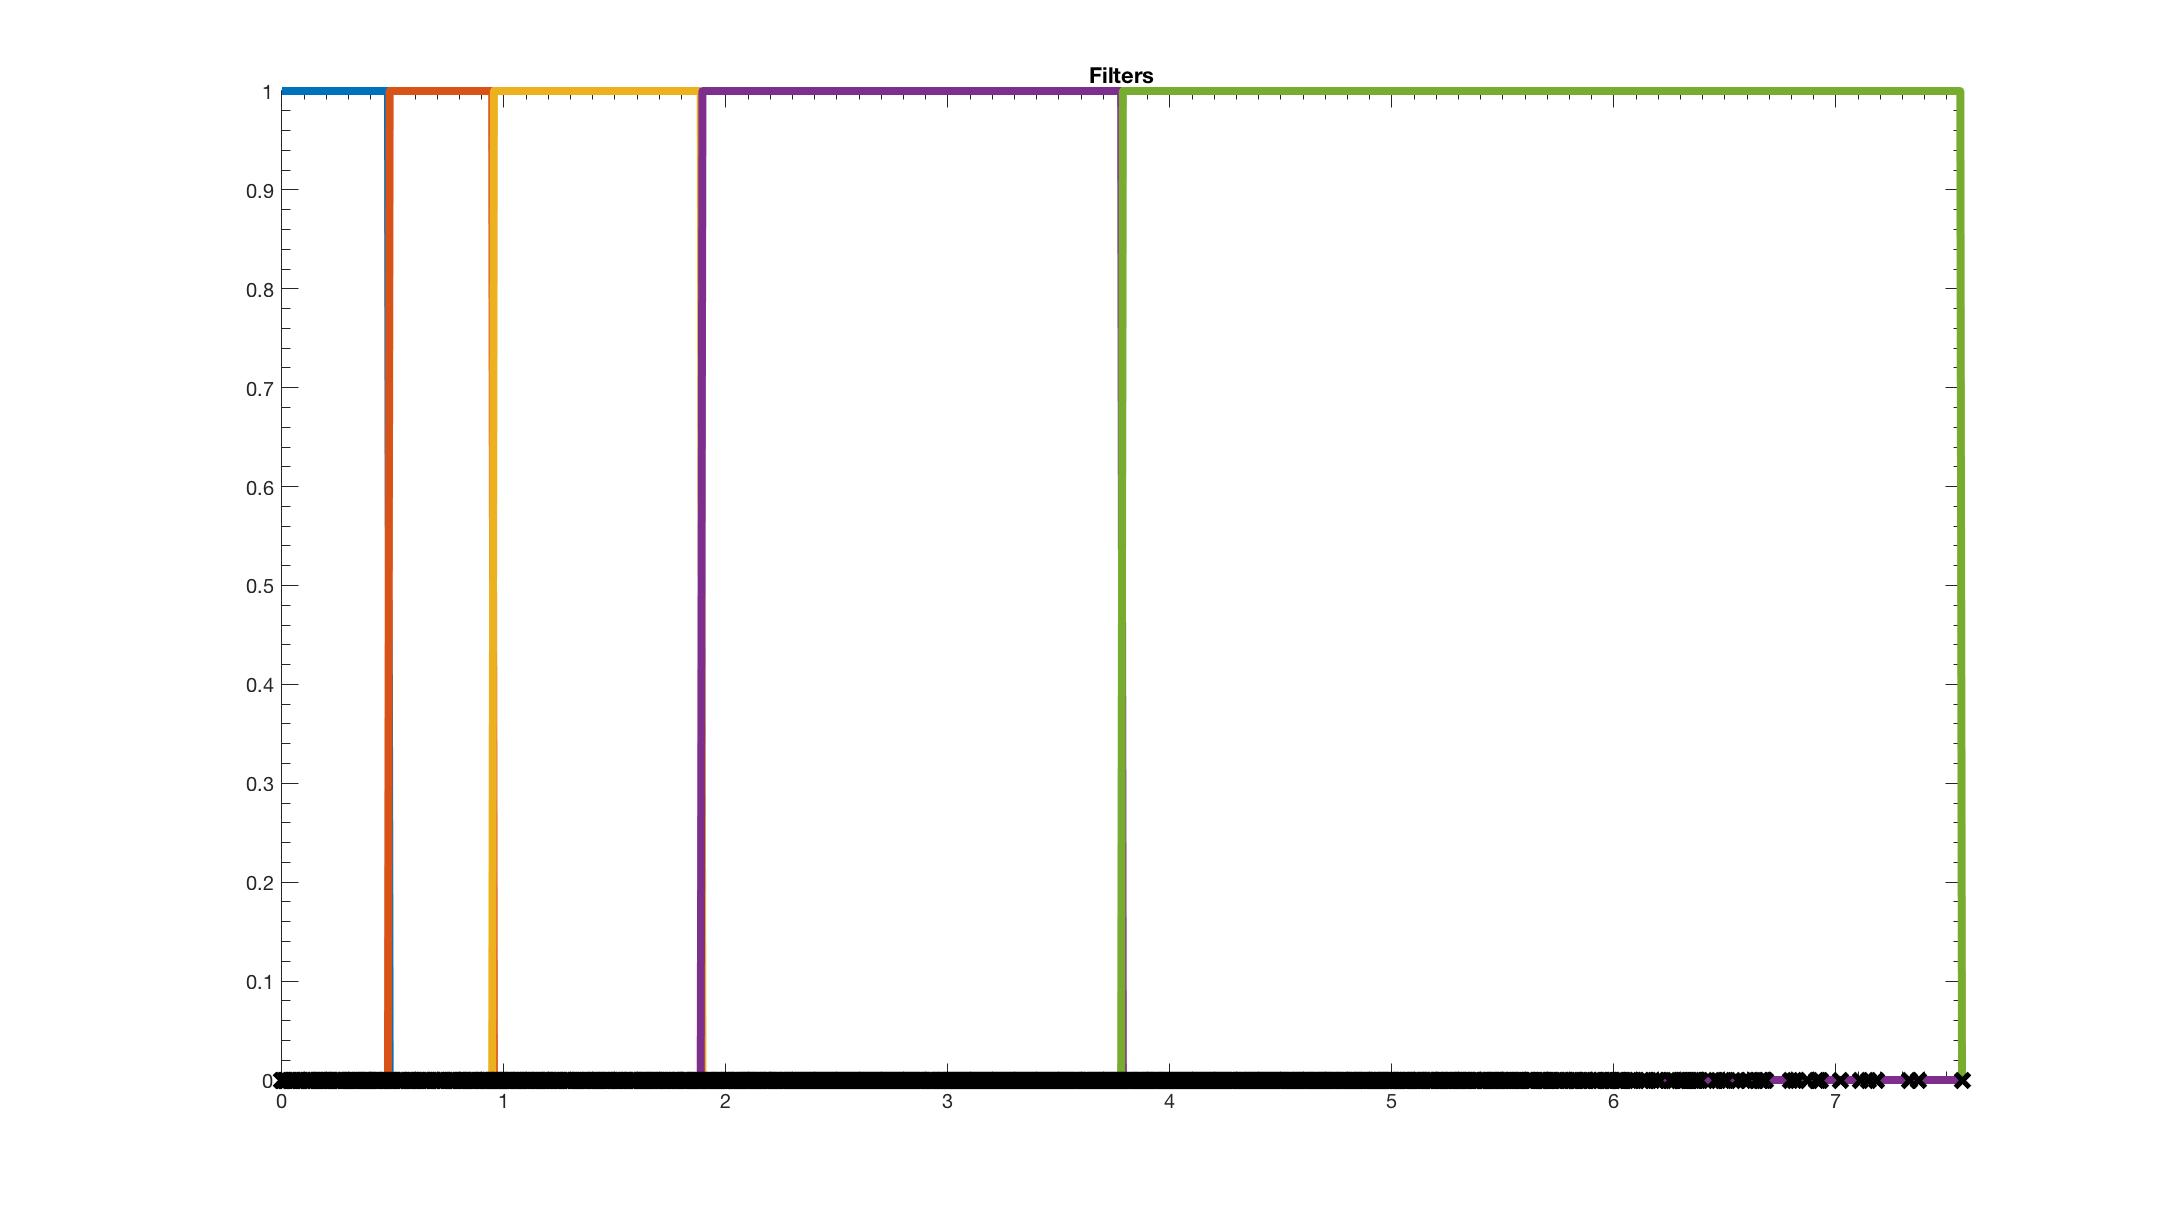
\includegraphics[width = 5cm]{filter_bank_4}
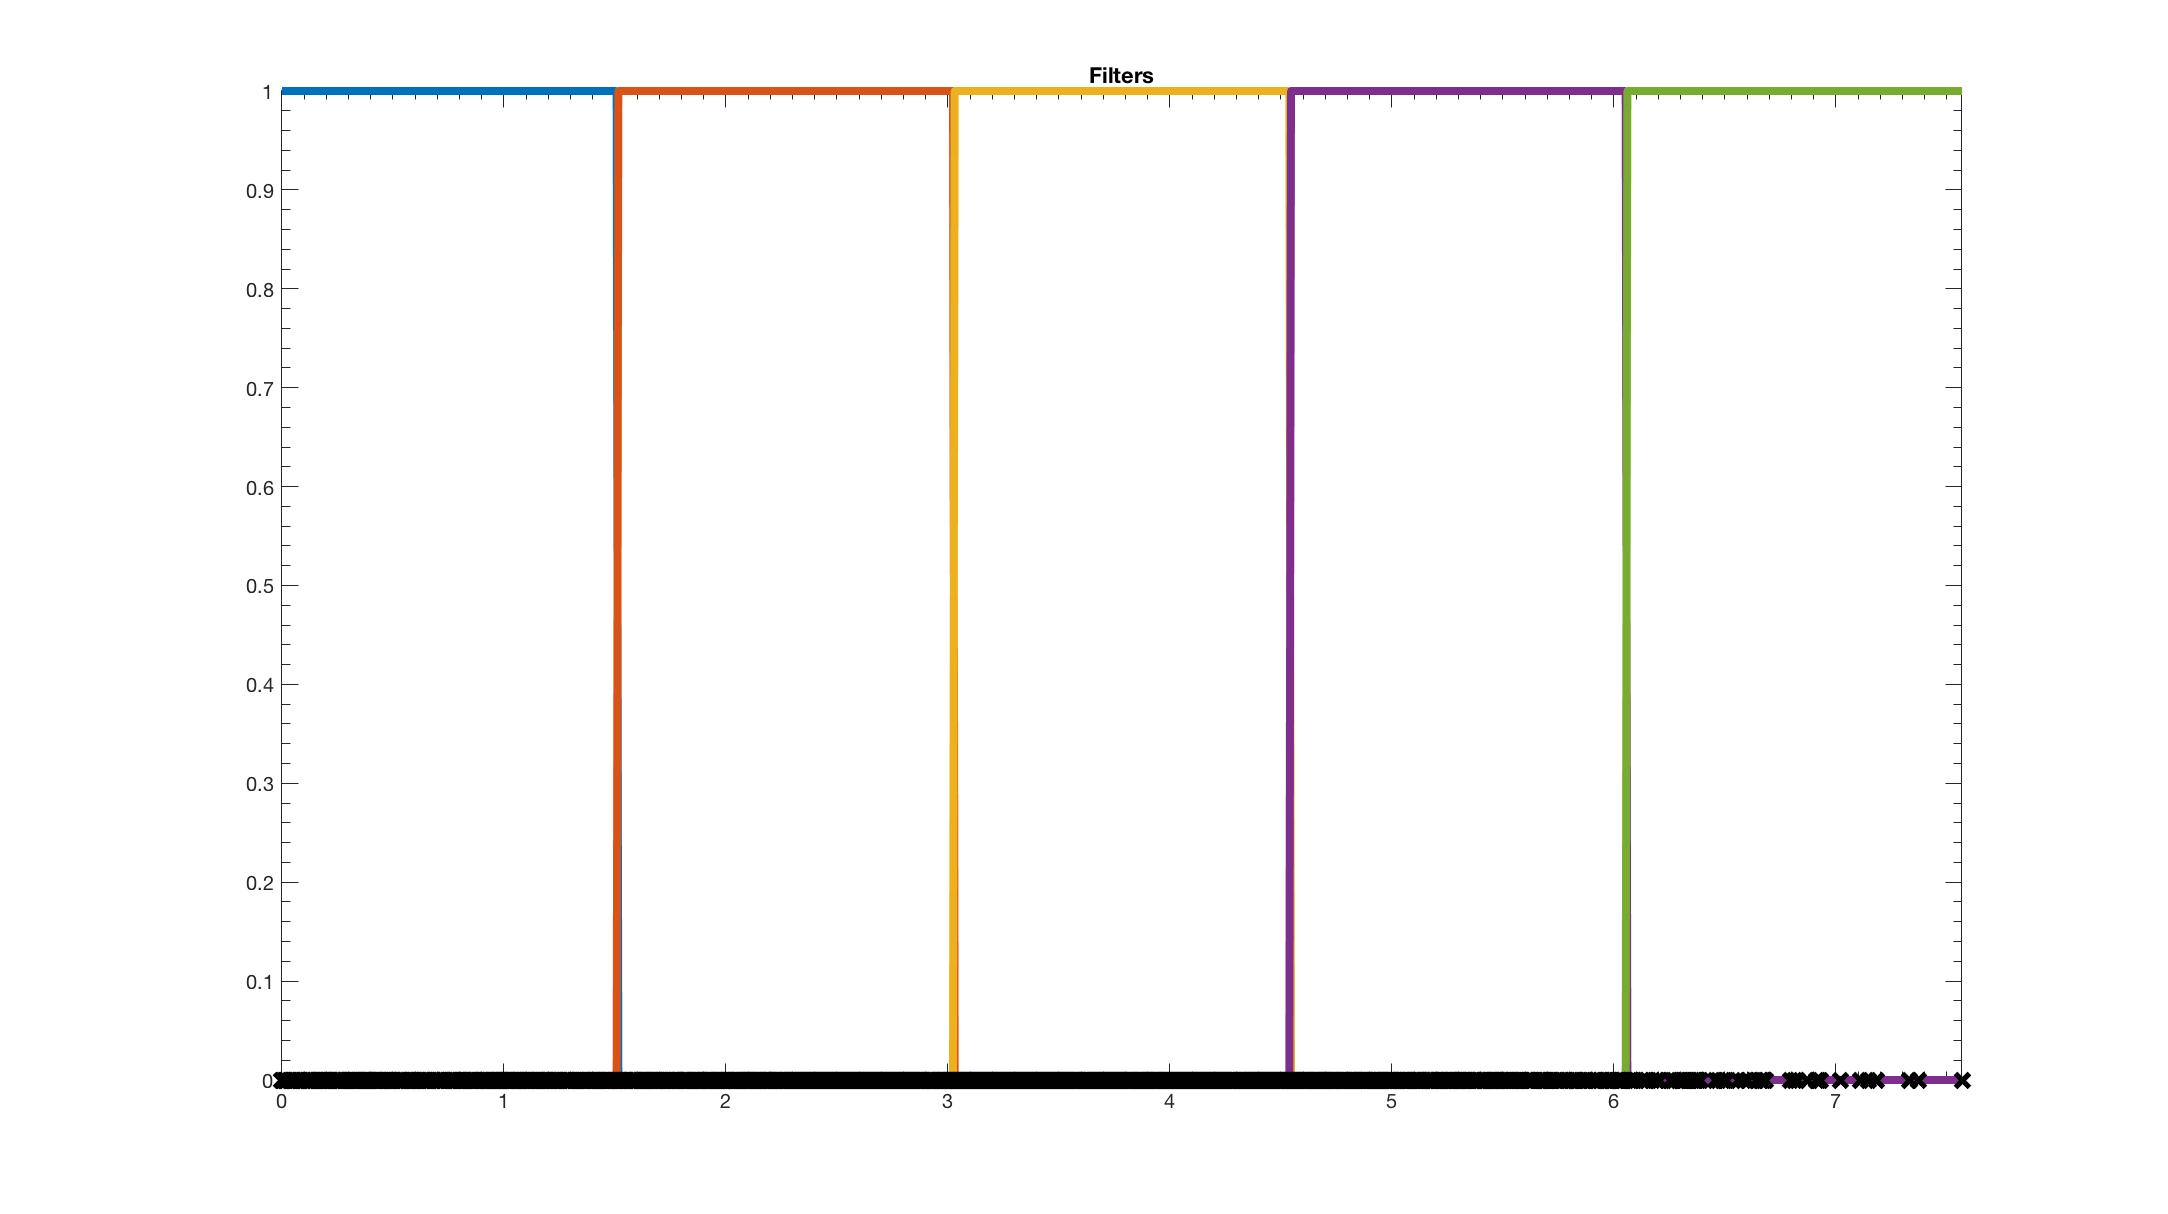
\includegraphics[width = 5cm]{filter_bank_3}


\caption{(a) is a spectrum-adapted and logarithmic spaced filter bank of 5 filters. Notice that this filter bank takes the density of Laplacian eigenvalues into account. The 4th filter covers half of the eigenvalues, the 3rd filter covers 1/4 of the eigenvalues, and each of the first two filters covers 1/8 of the eigenvalues.(b) stands for a spectrum-adapted but evenly spaced filter bank. Each of the five filters covers approximately the same number of eigenvalues. (c) and (d) are not spectrum-adapted. Notice that in this case the band ends only depend on the width of the spectrum.}
\end{figure}

Instead of storing the exact filters in Figure 1, we store the coefficients of Chebyshev and Jackson-Chebyshev polynomial approximations\cite{ShumanSIPN2018} and those coefficients will be applied to filter any given signal  \cite{shuman2013spectrum}.


\subsubsection{Adjust Band Ends to Minimize Approximation Error}

We first find the searching interval and search for the eigenvalue that has a mimimum pdf value in the range.
Our approach intends to spot spectral gaps and set the bands ends in the spectral gaps. The intuition behind this approach is to cluster the error around boundaries. If the boundaries are in spectral gaps, i.e. there are no eigenvalues around it, the error will not affect the approximated filters.


We use two examples to illustrate the usefulness of this idea:

1. ideal filter
2. approximated
3. in spectral gap
4. not in spectral gap\\


Let the $s$ be the width of the gap. We intend to find $x$ such that $F(s+x)F-(x)$ is minimized. That is, we want to minimized the probability of eigenvalues existing in the interval $[x, x+s]$.



{\color{blue}
\section{Non-Uniform Sampling and Reconstruction}
\begin{itemize}
\item Estimating number of measurements for each band
\item Review of non-uniform random sampling literature
\item Reconstruction - emphasize change from only lowpass bands
\item {\color{red} Solving the reconstruction equation efficiently and robustly}
\end{itemize}
}


\begin{thm}[\cite{puy}, Theorem 3.2]
Consider any graph $\G = \{\V, \E, W\}$ with its Laplacian $\La = U\Lambda U^*$. Notice that $\La$ is real, symmetric and positive semi-definite and thus the columns of U are orthonormal and its eigenvalues are non-negative. We propose the following sampling procedure:

\begin{enumerate}

\item Sampling Distribution. Let $\R \subseteq \{0,1,\cdots, n-1\}$. Define $\bm{p} \in \RR^n$ as the sampling distribution on vertices $\{1,2, \cdots n\}$  such that 

\[\bm{p_i} = \frac{||U^T_\R\bm{\delta_i}||^2_2}{|\R|} \text{, for } i = 1,2 ,\cdots, n. \tag{1}\]  
The sampling distribution $\bm{p}$ minimizes the graph weighted coherence. We associate the matrix $P = \text{diag}(\bm{p}) \in \RR^{n\times n}$.

\item Subsampling Matrix. Let $\Omega = \{\omega_1, \omega_2, \cdots, \omega_m\}$ be the subset of nodes drew independently from the set $\{1,2,\cdots n\}$ according to the sampling distribution $\bm{p}$. Define $M$ as the random subsampling matrix with the sampling distribution $\bm{p}$ such that

\[M_{ij} = 
\begin{cases} 
      1 & \text{ if } j = \omega_{i}\\
      0 & \text{otherwise}
   \end{cases}
\tag{2}\] 

for all $i \in \{1,2,\cdots,m\}$ and $j \in \{1,2,\cdots, n\}$.

\end{enumerate}

\medskip

From the $m$ samples obtained using the sampling method above, we can reconstruction all $\R$-concentrated signals accurately by solving the optimization problem 
\[\underset{\bm{f} \in \text{span}(\UR)}{\text{min}}\vert\vert P^{-1/2}_\Omega (M\bm{f}-\bm{y})\vert\vert_2, \tag{3}\] 
which estimates signal $\bm{f} \in \RR^n$ from $\bm{y} \in \RR^m$. 

Let $\epsilon, \delta \in (0,1)$. Let $\bm{f^*}$ be the solution of the problem (3). With probability at lease $1-\epsilon$, the following holds for all $\bm{f}\in \text{span}(U_{\R})$ and all $\bm{n}\in \RR^m: $

\[||x^* - x||_2 \leq \frac{2}{\sqrt{m(1-\delta)} ||P_{\Omega}^{-1/2} \bm{n}||_2} \tag{4}\]
provided that \[m \geq \frac{3}{\delta^2}\vv^k_{\bm{p}}\log(\frac{2k}{\epsilon}). \tag{5} \]

\end{thm}


{\color{blue}
\section{Illustrative Examples II: Approximate Calculations}
\begin{itemize}
\item Make sure to have some very large examples and show computation times
\end{itemize}
}







\end{document}